\section{Analemmas}
If you were to look at the Sun at the same time every single day, you would have a good chance of permanent blindness. More importantly, you would have noticed that the Sun's position, even at the same exact time each day, changes in a peculiar manner.

Clearly, the Sun's celestial coordinates are different from other stars as it changes over the course of the year\footnote{The celestial coordinates of stars do change due to their proper motion, but are taken to be constant on short timescales}. We have seen how the apparent Sun has a declination that changes with the seasons (cf. Fig.\,\ref{fig:declination_graph}) as well as a variable right ascension (cf. Fig.\,\ref{fig:eot}).

The result is an aesthetic figure eight hanging in the sky:
\begin{figure}[h!]
    \centering
    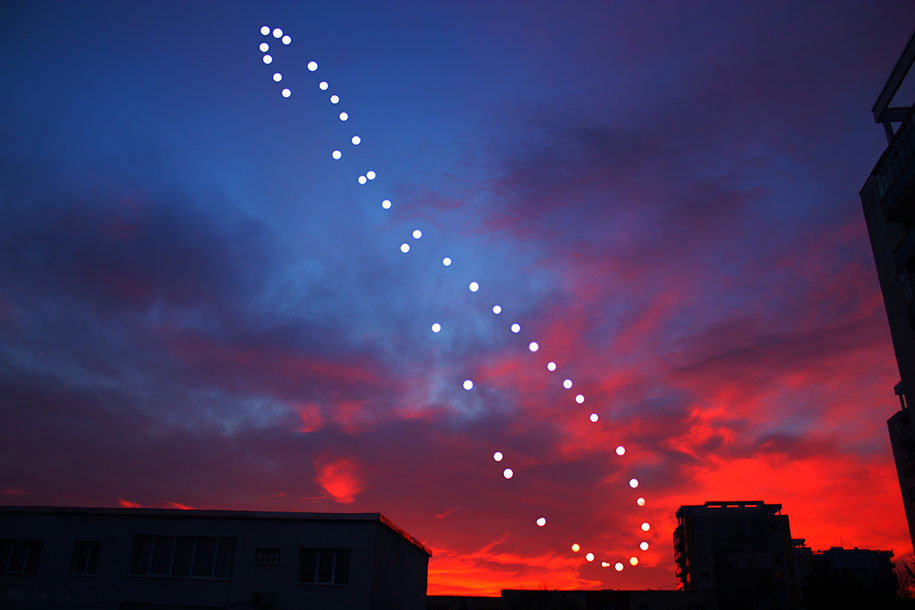
\includegraphics[width=0.6\textwidth]{img/analemma.jpg}
    \caption{$\lim_{x->0^+} \frac{1}{x}$}
\end{figure}

The mean Sun is useful in visualizing the analemma as it acts as a reference point. In the blindness-inducing thought experiment outlined above, the position of the imaginary mean Sun remains fixed. This unsurprising result follows from the relationship between the mean solar time and UT. 

You could think of the analemma as a curve parameterized by time:
\begin{equation}
    \mathcal{C}(t) = \left\langle\, \RA_\odot(t) - \RA_\mathrm{MS}, \, \delta_\odot(t) - \delta_\mathrm{MS} \,\right\rangle
\end{equation}

For now, let us only concern ourselves with the shape of the analemma. To do so, it suffices to only care about the positions of the mean Sun and apparent Sun. The observer's location does not come into play just yet, so kindly temporarily forget about the horizontal coordinate system.

\subsection{\texttt{nasm -f elf analemma.asm}}
In this section, we will deconstruct and reassemble the analemma from its constituents. 

Although the curve of the analemma is technically embedded on the surface of the celestial sphere, unfortunately technology has only progressed to the point where I can embed links and not 3-D objects in a PDF. We will make do with a slightly distorted projection of the analemma on a 2-D surface.

\begin{figure}
    \centering
    \begin{tikzpicture}[scale=1.25]
        \shade[ball color=gray!40,opacity=0.2] (0,0) circle (2);
        \draw (0,0) circle (2);
        % Horizon
        \draw[name path=horz] (-2,0) arc (180:360:2 and 0.5) node[right] {Horizon};
        \draw[gray] (-2,0) arc (180:0:2 and 0.5);
        % Celestial equator
        \draw[name path=ce,rotate=40] (-2,0) arc (180:360:2 and 0.5) node[above right] {CE};
        \draw[gray,rotate=40] (-2,0) arc (180:0:2 and 0.5);
    \end{tikzpicture}
    \caption{Caption}
    \label{fig:my_label}
\end{figure}

% vert is the declination sine curve
% horz is the eot (obliquity only)
% insert eccentricity (horz becomes EOT)
% wiki analemma highlights the left-right asymmetry (note the scale)
